\documentclass{beamer}

% ====================
% Packages
% ====================

\usepackage[T1]{fontenc}
\usepackage{lmodern}
\usepackage[size=custom,width=120,height=88,scale=1.0]{beamerposter}
\usetheme{gemini}
\usecolortheme{imsa}
\usepackage{graphicx}
\usepackage{booktabs}
\usepackage{tikz}
\usepackage{pgfplots}
\usepackage{fancyhdr}


% ====================
% Lengths
% ====================

% If you have N columns, choose \sepwidth and \colwidth such that
% (N+1)*\sepwidth + N*\colwidth = \paperwidth
\newlength{\sepwidth}
\newlength{\colwidth}
\setlength{\sepwidth}{0.025\paperwidth}
\setlength{\colwidth}{0.3\paperwidth}



\newcommand{\separatorcolumn}{\begin{column}{\sepwidth}\end{column}}

% ====================
% Title
% ====================


\title{Optimizing Trigger Selection for Detection of Doubly Charged Higgs Bosons at the LHC}

\author{Rohan Jain}

\institute[shortinst]{ {\texttt{rjain@imsa.edu} \\

Illinois Mathematics and Science Academy
}}
\logo{

\includegraphics[width=0.15\textwidth]{IMSAlogo.png}
\hspace{1.5cm}
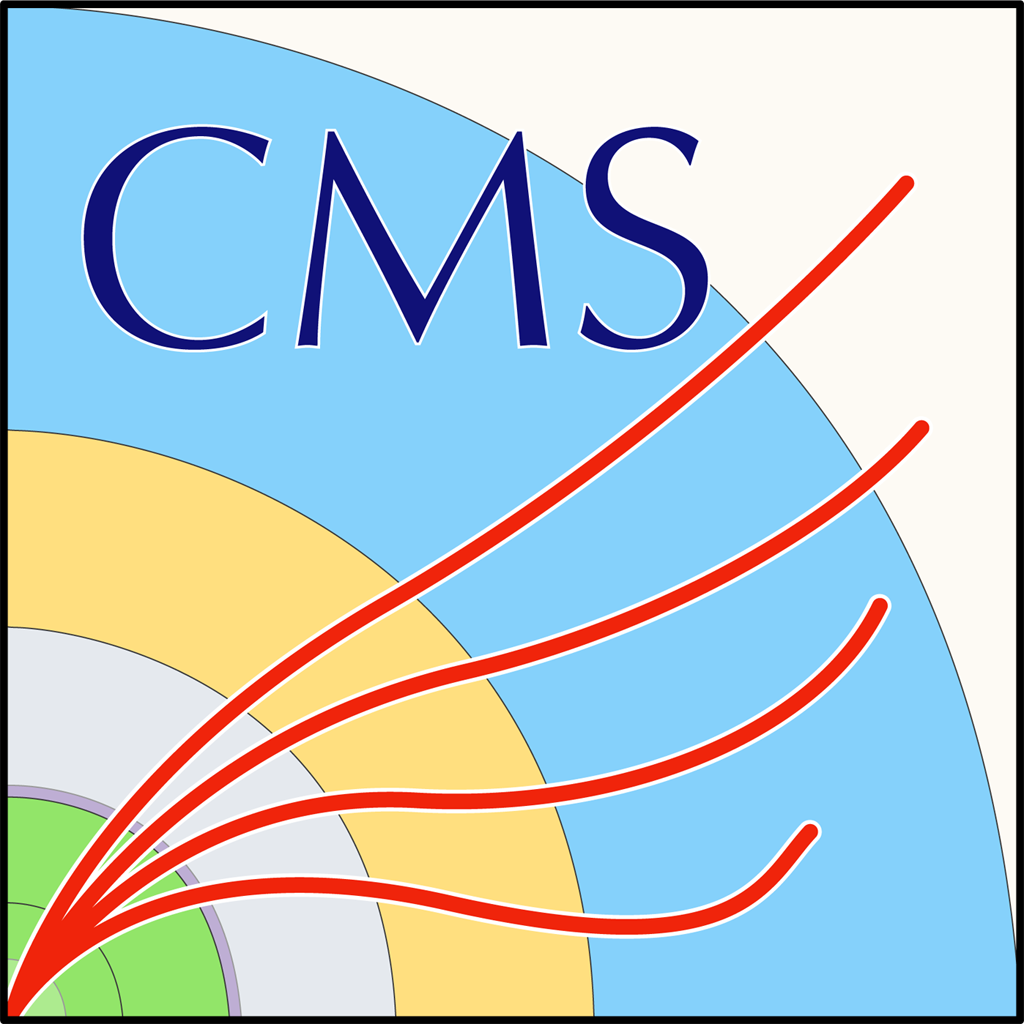
\includegraphics[]{CMSlogo.png}
}

% ====================
% Body
% ====================

\pgfplotsset{compat=1.18}

\begin{document}

\begin{frame}[t]
\begin{columns}[t]
\separatorcolumn

\begin{column}{\colwidth}
  \begin{block}{Abstract}
    In this project, we aim to programmatically find the most efficient triggers for selecting H++ events for application in the Compact Muon Solenoid experiment. Highly efficient triggers are defined as those with high signal efficiency and low background efficiency to give as much signal and as little background as possible. The types of events analyzed were H++, Drell-Yan, and QCD. The initial process started with finding the most efficient triggers on the three sets of events independently, then pairwise comparing the differences, and then finally creating a new figure of merit which was the harmonic mean of all the differences. 
  \end{block}

\begin{block}{Signal}
  The signal interaction we are searching for is activity of the double charged Higgs boson:

  \begin{itemize}
    \item H++: 
  \end{itemize}
\end{block}

  \begin{block}{Background}

    Background interactions include the following:

    \begin{itemize}
      \item Quantum Chromodynamics (QCD). QCD interactions are a strong interaction between quarks that are done through gluons. 
      \item Drell-Yan (DY). DY interactions occur when a quark and an antiquark of distinct hadrons annilhate, form a Z-boson, then decay into oppositely charged leptons.
    \end{itemize}
  \end{block}

  \begin{block}{Process}
    We start by running Monte Carlo data through a trigger simulation, enabling all triggers individually.

    \begin{itemize}
        \item H++
        \begin{itemize}
            \item Higgs900.txt
            \begin{itemize}
                \item $m$ of at least 900 GeV
            \end{itemize}
        \end{itemize}
        \item QCD
        \begin{itemize}
            \item QCD500-700.txt
            \begin{itemize}
                \item $H_T$ between 500-700 GeV
            \end{itemize}
        \end{itemize}
        \item Drell-Yan
        \begin{itemize}
            \item DY50.txt
            \begin{itemize}
                \item $m$ of at least 50 GeV
            \end{itemize}
        \end{itemize}
    \end{itemize}
  \end{block}

  \begin{block}{Preliminary Results}
    The tables below show the results for the top 5 triggers (highest efficiencies) for each of the three types of events.

    \begin{table}[]
      \begin{center}
           \caption{\label{table:1}Trigger Results for H++}
     \begin{tabular}[t]{c|c}
          \hline
          \textbf{Trigger Name} & \textbf{Efficiency}\\
          \hline
          HLT\_AK8PFJet40 & 0.999155\\
          HLT\_HcalPhiSym & 0.999 \\
          HLT\_AK4PFJet30 & 0.99879 \\
          HLT\_AK4CaloJet30 & 0.993445 \\
          HLT\_DiPFJetAve40  & 0.991245
      \end{tabular}
    \end{center}
    \end{table}
    \begin{table}
      \caption{\label{table:2}Trigger Results for QCD}
          \begin{tabular}[t]{c|c}
              \hline
              \textbf{Trigger Name} & \textbf{Efficiency}\\
              \hline
              HLT\_HcalPhiSym & 0.862971\\
              HLT\_AK8PFJet40 & 0.688192 \\
              HLT\_AK4CaloJet30 & 0.619257 \\
              HLT\_AK4PFJet30 & 0.598404 \\
              HLT\_PFJet40 & 0.465758
          \end{tabular}
  \end{table}

  \begin{table}[h!]
    \caption{\label{table:3}Trigger Results for DY}
        \begin{tabular}[t]{c|c}
            \hline
            \textbf{Trigger Name} & \textbf{Efficiency}\\
            \hline
            HLT\_HcalPhiSym & 0.884871\\
            HLT\_AK8PFJet200 & 0.882028 \\
            HLT\_HT425 & 0.872316 \\
            HLT\_PFJet200 & 0.773207 \\
            HLT\_DiPFJetAve200 & 0.546264
        \end{tabular}
\end{table}
    

  \end{block}

\end{column}

\separatorcolumn

\begin{column}{\colwidth}

  \begin{block}{Redefining Efficiency}

    Since we need to compare the efficiency of the same trigger across different events, we need to redefine the efficiency of a trigger. So when comparing H++ to any background, we will use the difference of efficiencies across mutual triggers. This can effectively be summarized with the following equation 

    $$i dont remmeber ngl$$
    
  \end{block}

  \begin{block}{Intermediary Results}
    The tables below show the results for the top 5 triggers (highest difference in efficiencies) for the pairwise comparisons of the three types of events.
    \begin{table}[h!]
      \caption{\label{table:4}Trigger Results for H++ vs. QCD}
          \begin{tabular}[t]{c|c}
              \hline
              \textbf{Trigger Name} & \textbf{Efficiency}\\
              \hline
              HLT\_DiPFJetAve320 & 0.81028139\\
              HLT\_PFJet320 & 0.8088902\\
              HLT\_PFMETNoMu110\_PFMHTNoMu110\_IDTight & 0.8054678 \\
              HLT\_Photon75 & 0.8039625 \\
              HLT\_Photon90 & 0.8035066 
          \end{tabular}
    \end{table}

    \begin{table}[h!]
      \caption{\label{table:5}Trigger Results for H++ vs. DY}
          \begin{tabular}[t]{c|c}
              \hline
              \textbf{Trigger Name} & \textbf{Efficiency}\\
              \hline
              HLT\_AK8PFJet140 & 0.94992018\\
              HLT\_DiPFJetAve80 & 0.9497367\\
              HLT\_PFJet140 & 0.94761912 \\
              HLT\_PFHT250 & 0.94691313 \\
              HLT\_DiPFJetAve140 & 0.94661373
          \end{tabular}
    \end{table}
  \end{block}

  \begin{block}{Redefining Efficiency (pt. 2)}
    To compare values in the two tables above, we need to redefine efficiency again. This time, we will use the following equation:

    $$Efficiency = \frac{1}{\frac{1}{Eff_{H++ vs. QCD}} + \frac{1}{Eff_{H++ vs. DY}}}$$
  \end{block}

  \begin{block}{Final Results}
    The tables below shows the (i honestly dont remember)

    \begin{table}[h!]
      \caption{\label{table:6}Trigger Results for H++ vs. DY \& QCD}
          \begin{tabular}[t]{c|c}
              \hline
              \textbf{Trigger Name} & \textbf{Efficiency}\\
              \hline
              HLT\_PFJet320 & 1.6658838 \\
              HLT\_Photon75 & 1.6451807 \\
              HLT\_AK8PFJet320 & 1.6429796 \\
              HLT\_Photon90 & 1.64207 \\
              HLT\_DiPFJetAve260 & 1.632191
          \end{tabular}
  \end{table}

  \begin{table}[h!]
    \caption{\label{table:6}Trigger Results for H++ vs. DY \& QCD}
        \begin{tabular}[t]{c|c}
            \hline
            \textbf{Trigger Name} & \textbf{Harmonic Mean $/$ $n$}\\
            \hline
                HLT\_PFJet500 & 9591.97113454199 \\
                HLT\_CaloJet500\_NoJetID & 9304.47172437449 \\
                HLT\_DiPFJetAve400 & 8315.637583350732 \\
                HLT\_AK8PFJet500 & 7420.99538836046 \\
                HLT\_Ele300\_CaloIdVT\_GsfTrkIdT & 6862.191246355468
        \end{tabular}
\end{table}
  \end{block}

\end{column}

\separatorcolumn

\begin{column}{\colwidth}

  \begin{block}{Questions}



  \end{block}
  \begin{block}{Next Steps}

  \end{block}
  \begin{block}{Conclusions}

  \end{block}


 % \begin{block}{References}

    %\nocite{*}
    %\footnotesize{\bibliographystyle{plain}\bibliography{poster}}

  %\end{block}

\end{column}

\separatorcolumn
\end{columns}
\end{frame}

\end{document}